\documentclass[11pt, a4paper, twoside, openright]{book}
\usepackage{subfiles}

% Algorithms
	%\usepackage{algpseudocode}
	%\usepackage{algorithm}

% Babel
\usepackage[english]{babel}

% Code writing
	%\usepackage[procnames]{listings}

% Font
\usepackage[utf8]{inputenc}
\usepackage[T1]{fontenc}
\usepackage{amssymb,amsmath,amsthm,amsfonts}
\usepackage{eucal}
\usepackage{textcomp}

% Footnote


% Hyperref
\usepackage[hyphens]{url}
\usepackage{cite}
\usepackage{hyperref}
\usepackage{nameref}

% Images
\usepackage[pdftex]{graphicx}
	%\usepackage{subfigure}
\usepackage{subfig}
\usepackage{eso-pic}
\usepackage{caption}
\usepackage{wrapfig}

% List
\usepackage{enumerate}

% SI units
\usepackage{siunitx}

% Standalone
\usepackage[subpreambles=true]{standalone}
\usepackage{import}

% Tables
\usepackage{tabularx}
\usepackage{booktabs}
\usepackage{multirow}

% TiKz and graphs
\usepackage{pgf,tikz,pgfplots}
% \usepackage{gnuplottex}
\usepackage{bm}
\usepackage{relsize}
%\usepackage[compat=1.1.0]{tikz-feynman}
\usepackage{circuitikz}

% Typeset
%\usepackage[top=2cm,bottom=2cm,left=2cm,right=2cm]{geometry}
\usepackage[top=2cm,bottom=2cm,left=2cm,right=2cm,headheight=13.6pt]{geometry}
\usepackage{fancyhdr}
\usepackage{indentfirst}
\usepackage{titlesec}
\usepackage{setspace}
\usepackage{xspace}
% \usepackage{parskip}  % Elimina il separatore a inizio paragrafo
\usepackage{afterpage}
\usepackage{comment}

%Python
\usepackage{xcolor}
\usepackage{listings}
\usepackage{framed}

%Per scrivere matrice identità
\usepackage{bbold}
%Per semplificazione formule
\usepackage{cancel}

%Evidenziare formule
\usepackage{empheq}
	%oppure
	%\usepackage{xcolor}
\usepackage{soul}

%Evidenziare testo con mdframed
\usepackage{mdframed}

%Note a margine
\usepackage{marginnote}

%Display data
\usepackage{datetime}

%Physics
% \usepackage{physics}

%Marginpar in the correct side
\usepackage{mparhack}

%Geometry
\newgeometry{inner=20mm,
            outer=49mm,% = marginparsep + marginparwidth
                       %   + 5mm (between marginpar and page border)
            top=20mm,
            bottom=25mm,
            marginparsep=6mm,
            marginparwidth=30mm}
\makeatletter
\renewcommand{\@marginparreset}{%
  \reset@font\small
  \raggedright
  \slshape
  \@setminipage
}
\makeatother

%Atom Latex
\pgfplotsset{compat=1.15}

%%
\captionsetup[table]{font=small,labelfont={bf},skip=10pt}
\captionsetup[figure]{font=small,labelfont={bf},skip=10pt}

%intestazione pagina
\pagestyle{fancy}
\fancyhf{}
\fancyhead[RE]{\ifnum\value{chapter}>0\nouppercase{\leftmark}\fi}
\fancyhead[LE]{\small\textbf{\thepage}}
\fancyhead[LO]{\nouppercase{\rightmark}}
\fancyhead[RO]{\small\textbf{\thepage}}

%link ipertestuale per indice
\hypersetup{
	colorlinks=false,
	linkcolor=black,
	filecolor=blue,
	citecolor = blue,
	urlcolor=blue,
	}

%%%%%indent%%%
\setlength{\parindent}{15pt}
\setlength{\parskip}{0pt}


%boh
\renewcommand{\chaptermark}[1]{%
 \markboth{\MakeUppercase{%
 \chaptername}\ \thechapter.%
 \ #1}{}}


 %Python in latex
 \definecolor{codegreen}{rgb}{0,0.6,0}
\definecolor{codegray}{rgb}{0.5,0.5,0.5}
\definecolor{codepurple}{rgb}{0.58,0,0.82}
\definecolor{backcolour}{rgb}{0.95,0.95,0.92}
\definecolor{commentcolour}{rgb}{0.43,0.63,0.65}

\definecolor{shadecolor}{rgb}{0.93, 0.93, 0.93}
\definecolor{darkgreen}{rgb}{0.0, 0.5, 0.0}
\definecolor{darkred}{rgb}{0.8, 0.0, 0.0}
\definecolor{violet}{rgb}{0.55, 0.0, 0.55}
%
%\lstdefinestyle{mystyle}{ %Stile python code
%    backgroundcolor=\color{shadecolor},
%    commentstyle=\color{commentcolour},
%    keywordstyle=\color{darkgreen},
%    numberstyle=\tiny\color{codegray},
%    stringstyle=\color{darkred},
%    basicstyle=\ttfamily\footnotesize,
%    breakatwhitespace=false,
%    breaklines=true,
%    captionpos=b,
%    keepspaces=true,
%    numbers=left,
%    numbersep=5pt,
%    showspaces=false,
%    showstringspaces=false,
%    showtabs=false,
%    tabsize=2
%}

\definecolor{cadmiumred}{rgb}{0.89, 0.0, 0.13}

%\lstdefinestyle{mystyle}{ %Stile python code
%    backgroundcolor=\color{white},
%    commentstyle=\color{commentcolour},
%    keywordstyle=\color{cadmiumred},
%    numberstyle=\tiny\color{codegray},
%    stringstyle=\color{darkgreen},
%    basicstyle=\ttfamily\footnotesize,
%    breakatwhitespace=false,
%    breaklines=true,
%    captionpos=b,
%    keepspaces=true,
%    numbers=left,
%    numbersep=5pt,
%    showspaces=false,
%    showstringspaces=false,
%    showtabs=false,
%    tabsize=2
%}

\usepackage{inconsolata} %To change the font of the listings to the one of Atom

\lstdefinestyle{Fortran}{language=Fortran,    
    backgroundcolor=\color{white},
    commentstyle=\color{commentcolour},
    keywordstyle=\bfseries\color{cadmiumred},
    numberstyle=\tiny\color{codegray},
    stringstyle=\color{darkgreen},
    basicstyle=\ttfamily\footnotesize,
    breakatwhitespace=false,
    breaklines=true,
    captionpos=b,
    keepspaces=true,
    numbers=left,
    numbersep=5pt,
    showspaces=false,
    showstringspaces=false,
    showtabs=false,
    tabsize=2
}


\lstdefinestyle{Gnuplot}{ 
    backgroundcolor=\color{white},
    commentstyle=\color{commentcolour},
    basicstyle=\ttfamily\footnotesize,
    breakatwhitespace=false,
    breaklines=true,
    captionpos=b,
    keepspaces=true,
    showspaces=false,
    showstringspaces=false,
    showtabs=false,
    tabsize=2
}

\lstdefinestyle{Python}{language=Python,    
    backgroundcolor=\color{shadecolor},
    commentstyle=\color{commentcolour},
    keywordstyle=\color{darkgreen},
    numberstyle=\tiny\color{codegray},
    stringstyle=\color{darkred},
    basicstyle=\ttfamily\footnotesize,
    breakatwhitespace=false,
    breaklines=true,
    captionpos=b,
    keepspaces=true,
    numbers=left,
    numbersep=5pt,
    showspaces=false,
    showstringspaces=false,
    showtabs=false,
    tabsize=2
}

%\lstset{style=mystyle}




% Derivatives
\renewcommand{\d}[0]{\mathrm{d}}
\newcommand{\dev}[2]{\displaystyle \frac{\d #1}{\d #2}}
\newcommand{\pdev}[2]{\displaystyle \frac{\partial #1}{\partial #2}}
\newcommand{\ndev}[3]{\displaystyle \frac{\d^{#3} #1}{\d #2^{#3} } }
\newcommand{\npdev}[3]{\displaystyle \frac{\partial^{#3} #1}{\partial #2^{#3} } }


%% Norms
\newcommand{\absvec}[1]{| \vec{#1} |}
\newcommand{\normvec}[1]{|\!| \vec{#1} |\!|}

\newcommand{\vmed}[1]{\left \langle #1 \right \rangle}
\newcommand{\vmedvec}[1]{\langle #1 \rangle}
\newcommand{\R}[0]{\mathbb{R}}
\renewcommand{\H}[0]{\operatorname{H}}

%Evidenziare formule
\newcommand{\mathcolorbox}[2]{\colorbox{#1}{$\displaystyle #2$}}
\newcommand{\hlfancy}[2]{\sethlcolor{#1}\hl{#2}}

%letters above equal signs
\newcommand{\myeq}[1]{\mathrel{\overset{\makebox[0pt]{\mbox{\normalfont (#1)}}}{=}}}


%%%%%%%%%%%%%%%%%%%%Theorem, Corollary, Lemma, Proposition%%%%%%%%%%%%%%%%%
\usepackage[many,most,theorems]{tcolorbox}

\newtcbtheorem{theorem}{Theorem}{ % frame stuff
    boxrule = 1pt,
    breakable,
    enhanced,
    frame empty,
    interior style= {orange!20},
    %interior empty,
    colframe=black,
    borderline ={1pt}{0pt}{black},
    left=0.2cm,
    % title stuff
    attach boxed title to top left={yshift=-2mm,xshift=0mm},
    coltitle=black,
    fonttitle=\bfseries,
    colbacktitle=white,
    fontupper=\slshape,
    boxed title style={boxrule=1pt,sharp corners}}{theorem} 

\newtcbtheorem{corollary}{Corollary}{ % frame stuff
    boxrule = 1pt,
    breakable,
    enhanced,
    frame empty,
    interior style= {orange!20},
    %interior empty,
    colframe=black,
    borderline ={1pt}{0pt}{black},
    left=0.2cm,
    % title stuff
    attach boxed title to top left={yshift=-2mm,xshift=0mm},
    coltitle=black,
    fonttitle=\bfseries,
    colbacktitle=white,
    fontupper=\slshape,
    boxed title style={boxrule=1pt,sharp corners}}{corollary} 
    
\newtcbtheorem{lemma}{Lemma}{ % frame stuff
    boxrule = 1pt,
    breakable,
    enhanced,
    frame empty,
    interior style= {orange!20},
    %interior empty,
    colframe=black,
    borderline ={1pt}{0pt}{black},
    left=0.2cm,
    % title stuff
    attach boxed title to top left={yshift=-2mm,xshift=0mm},
    coltitle=black,
    fonttitle=\bfseries,
    colbacktitle=white,
    fontupper=\slshape,
    boxed title style={boxrule=1pt,sharp corners}}{lemma} 


%%%%%%%%%%%%%%%%%%%%Definition%%%%%%%%%%%%%%%%%


\newtcbtheorem{definition}{Definition}{ % frame stuff
    boxrule = 1pt,
    breakable,
    enhanced,
    frame empty,
    interior style= {blue!10},
    %interior empty,
    colframe=black,
    borderline ={1pt}{0pt}{black},
    left=0.2cm,
    % title stuff
    attach boxed title to top left={yshift=-2mm,xshift=0mm},
    coltitle=black,
    fonttitle=\bfseries,
    colbacktitle=white,
    boxed title style={boxrule=1pt,sharp corners}}{definition} 


%\theoremstyle{definition}
%\newtheorem{definition}{Definition}%[section]



%%%%%%%%%%%%%%%%%%%%Exercise and example%%%%%%%%%%%%%%%%%

\newtcbtheorem{exercise}{Exercise}{ % frame stuff
    boxrule = 1pt,
    breakable,
    enhanced,
    frame empty,
    interior style= {blue!6},
    %interior empty,
    colframe=black,
    borderline ={1pt}{0pt}{black},
    left=0.2cm,
    % title stuff
    attach boxed title to top left={yshift=-2mm,xshift=0mm},
    coltitle=black,
    fonttitle=\bfseries,
    colbacktitle=white,
    boxed title style={boxrule=1pt,sharp corners}}{exercise} 

\newtcbtheorem{example}{Example}{ % frame stuff
    boxrule = 1pt,
    enhanced,
    frame empty,
    interior style= {green!6},%{left color=yellow!70,right color=green!70},
    %interior empty,
    colframe=black,
    borderline ={1pt}{0pt}{black},
    breakable,
    left=0.2cm,
    % title stuff
    attach boxed title to top left={yshift=-2mm,xshift=0mm},
    coltitle=black,
    fonttitle=\bfseries,
    colbacktitle=white,
    boxed title style={boxrule=1pt,sharp corners}}{example}

\theoremstyle{remark}
\newtheorem*{remark}{Remark}

%Evidenziare testo

\newcommand\mybox[1]{%
  \fbox{\begin{minipage}{0.9\textwidth}#1\end{minipage}}}

  %Spiegazioni/verifiche
\newenvironment{greenbox}{\begin{mdframed}[hidealllines=true,backgroundcolor=green!20,innerleftmargin=3pt,innerrightmargin=3pt]}{\end{mdframed}}

\newenvironment{bluebox}{\begin{mdframed}[hidealllines=true,backgroundcolor=blue!10,innerleftmargin=3pt,innerrightmargin=3pt]}{\end{mdframed}}

\newenvironment{yellowbox}{\begin{mdframed}[hidealllines=true,backgroundcolor=yellow!20,innerleftmargin=3pt,innerrightmargin=3pt]}{\end{mdframed}}

\newenvironment{redbox}{\begin{mdframed}[hidealllines=true,backgroundcolor=red!20,innerleftmargin=3pt,innerrightmargin=3pt]}{\end{mdframed}}

\newenvironment{orangebox}{\begin{mdframed}[hidealllines=true,backgroundcolor=orange!20,innerleftmargin=3pt,innerrightmargin=3pt]}{\end{mdframed}}

%emph equation
\newcommand*\myyellowbox[1]{%
  \colorbox{yellow!40}{\hspace{1em}#1\hspace{1em}}}

 % “Inspirational” quote at start of chapter
  \makeatletter
\renewcommand{\@chapapp}{}% Not necessary...
\newenvironment{chapquote}[2][2em]
  {\setlength{\@tempdima}{#1}%
   \def\chapquote@author{#2}%
   \parshape 1 \@tempdima \dimexpr\textwidth-2\@tempdima\relax%
   \itshape}
  {\par\normalfont\hfill--\ \chapquote@author\hspace*{\@tempdima}\par\bigskip}
\makeatother





%\usepackage{eso-pic}
%
%\newcommand\BackgroundPic{%
%\put(0,0){%
%\parbox[b][\paperheight]{\paperwidth}{%
%\vfill
%\centering
%\includegraphics[scale=1.5]{../frontespizio/back.jpg}%
%\vfill
%}}}

%\includegraphics[width=1.4\paperwidth,height=\paperheight,%
%keepaspectratio]{../frontespizio/back.jpg}

\begin{document}

%%%%%%FRONTESPIZIO%%%%%%
%Reset the geometry of frontespizio
\newgeometry{inner=20mm,
            outer=20mm,% = marginparsep + marginparwidth
                       %   + 5mm (between marginpar and page border)
            top=20mm,
            bottom=20mm,
            marginparsep=6mm,
            marginparwidth=30mm,
            headheight=13.6pt}
\makeatletter
\renewcommand{\@marginparreset}{%
  \reset@font\small
  \raggedright
  \slshape
  \@setminipage
}
\makeatother


\frontmatter

%\pagecolor{blue} %Page color blue!70
%%%%%%FRONTESPIZIO%%%%%%
\begin{titlepage} % Suppresses headers and footers on the title page

	\newcommand{\HRule}{\rule{\linewidth}{0.5mm}} % Defines a new command for horizontal lines, change thickness here
	
	\center % Centre everything on the page
	
	%------------------------------------------------
	%	Headings
	%------------------------------------------------
	
	\textsc{\LARGE University of Padova}\vspace{1.5cm} % Main heading such as the name of your university/college
	
	%------------------------------------------------
	%	Title
	%------------------------------------------------
	
	\HRule \vspace{0.5cm}
	
	\textbf{\LARGE LECTURE NOTES\\ OF\\ BIOLOGICAL PHYSICS\\} % Title
	\vspace{0.5cm}
	\HRule\\[0.5cm]
	
	\vspace{2\baselineskip} % Whitespace after the title block
	
	%------------------------------------------------
	%	Subtitle
	%------------------------------------------------
	
	\textsc{ \small Collection of the lectures notes of professor Fulvio Baldovin. }% Subtitle or further description
	
	\vspace*{3\baselineskip} % Whitespace under the subtitle
	
	%------------------------------------------------
	%	Editor(s)
	%------------------------------------------------
	
	Edited By
	
	\vspace{0.5\baselineskip} % Whitespace before the editors
	
	\textsc{ \Large Riccardo Tancredi \\} % Editor list
	
	\vspace{0.5\baselineskip} % Whitespace below the editor list
	
	\vspace{2cm}
	
	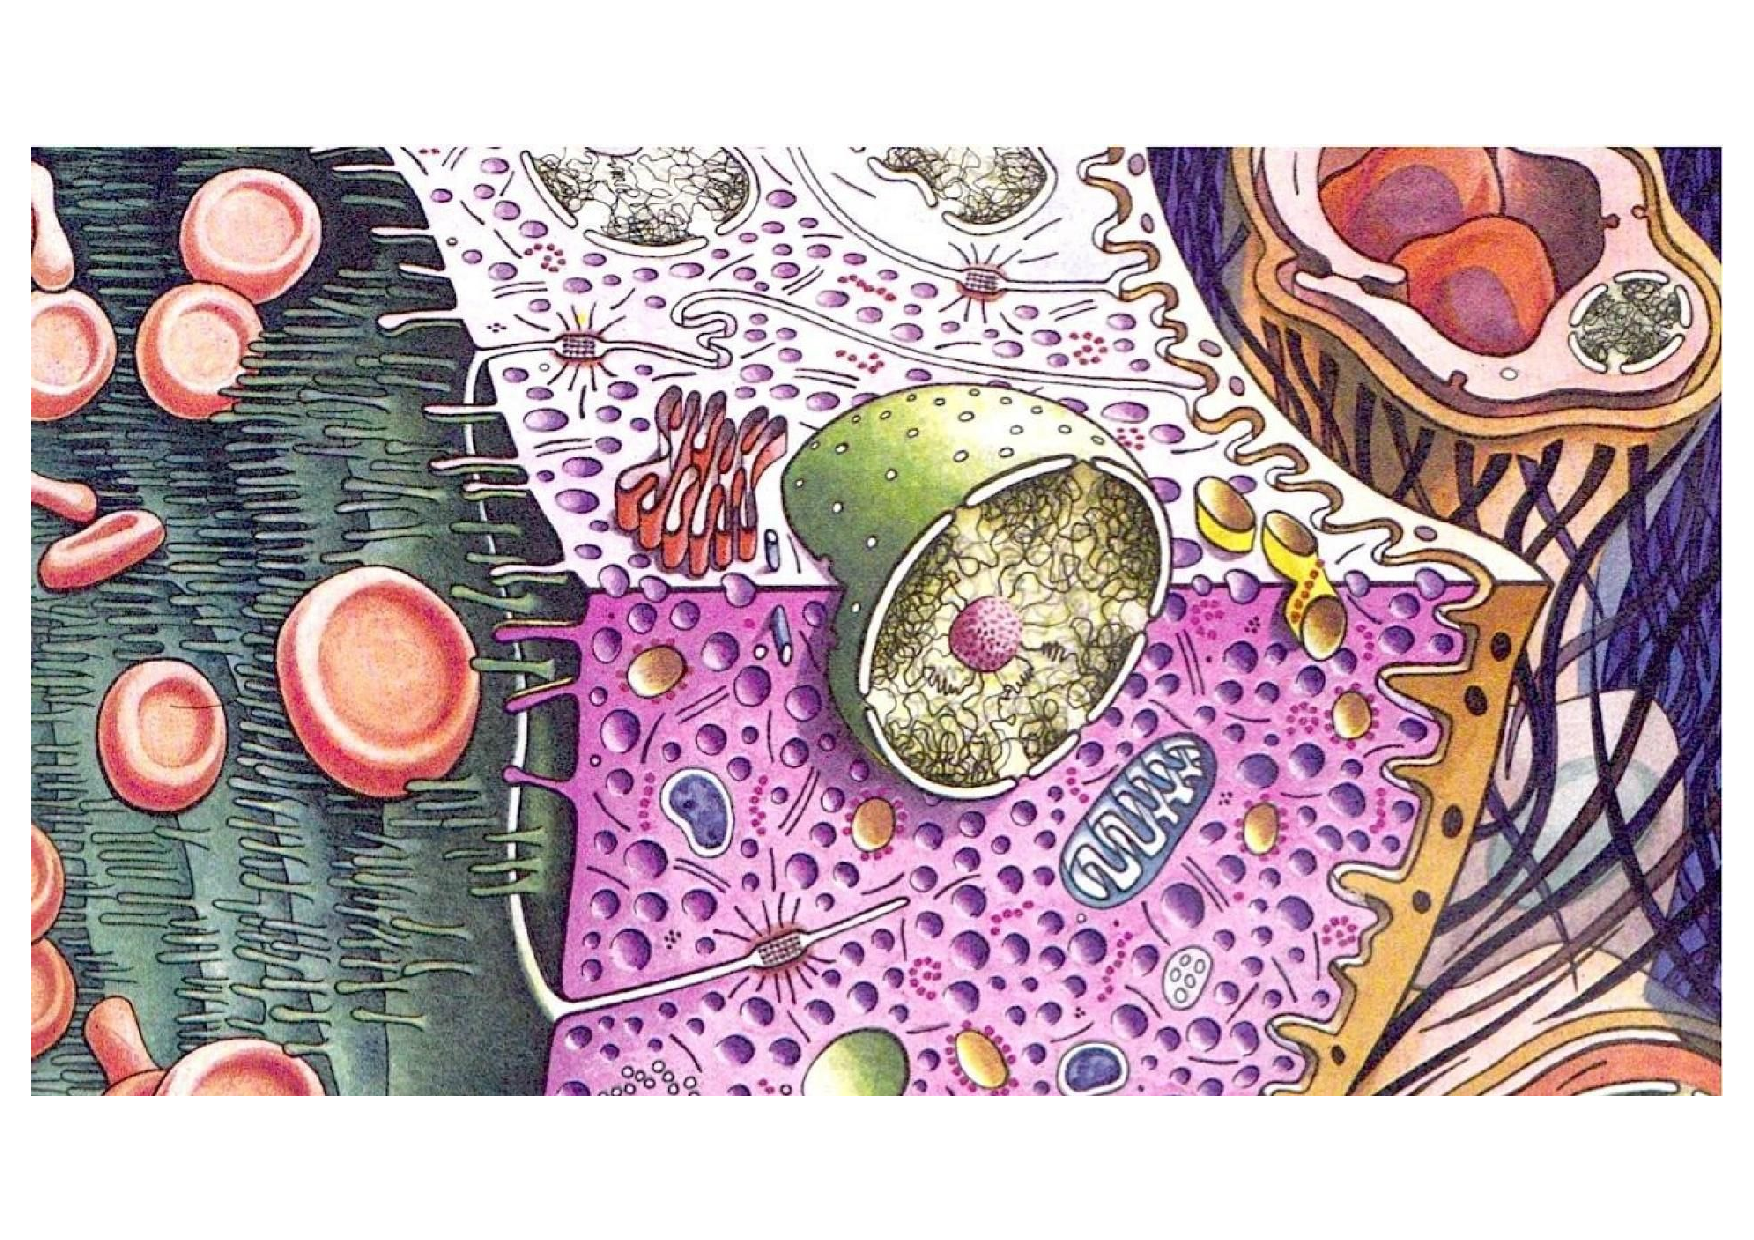
\includegraphics[width=15cm]{../frontespizio/figure.pdf}
	
	\vspace{2cm}
	
	\vfill % Whitespace between editor names and publisher logo
	
%	%------------------------------------------------
%	%	Publisher
%	%------------------------------------------------
%	
%	\plogo % Publisher logo
%	
%	\vspace{0.3\baselineskip} % Whitespace under the publisher logo
%	
%	2017 % Publication year
%	
%	{\large publisher} % Publisher

\end{titlepage}

\clearpage{\pagestyle{empty}\cleardoublepage}


%\pagecolor{white}

%%%ABSTRACT%%%%%%%%%

%\chapter*{\centering {\normalsize Abstract}}
%\noindent In this document I have tried to reorder the notes of the “Biological Physics” course held by Professor Fulvio Baldovin at the Department
%of Physics of the University of Padua during the second semester of the 2022-23 academic year of the master's degree.
%%The notes are \textbf{fully} integrated with the material provided by the professor in the Moodle platform.
%%In addition, I will integrate them, as best as possible, with the books recommended by the professor.
%There may be formatting errors, wrong marks, missing exponents etc. If you find errors, let me know (riccardo.tancredi@studenti.unipd.it) and I will correct them, so that this document can be a good study support.
%
%\vspace{1cm}
%\noindent Padova, \today  \hspace{6cm} Alice Pagano

\tableofcontents


\pagestyle{plain}

\newgeometry{inner=20mm,
            outer=49mm,% = marginparsep + marginparwidth
                       %   + 5mm (between marginpar and page border)
            top=20mm,
            bottom=25mm,
            marginparsep=6mm,
            marginparwidth=30mm}
\makeatletter
\renewcommand{\@marginparreset}{%
  \reset@font\small
  \raggedright
  \slshape
  \@setminipage
}
\makeatother





\mainmatter
\pagestyle{fancy}


% \part{Theory Lectures}

\subfile{../lessons/00_02-03-2023.tex}
\subfile{../lessons/01_03-03-2023.tex}
\subfile{../lessons/02_08-03-2023.tex}


\backmatter
\pagestyle{plain}

%\chapter{Conclusions}

%%%BIBLIOGRAFIA%%%

\cleardoublepage
\addcontentsline{toc}{chapter}{\bibname}
\begin{thebibliography}{99}

% \bibitem{Nielsen}
% Michael A. Nielsen and Isaac L. Chuang.
% \textit{Quantum computation and quantum information}.
% United Kingdom, Cambridge University Press, 2016.
%
%\bibitem{Divincenzo}
%David P. DiVincenzo
%\textit{The Physical Implementation of Quantum Computation}.
%IBM T.J. Watson Research Center, Yorktown Heights, NY 10598 USA
%February 1, 2008.
%arXiv:quant-ph/0002077
%
%\bibitem{DocumentationQiskit}
%The Qiskit Developers.
%\textit{Qiskit API documentation}.
%Release 0.8.0, 9 March 2019.
%\url{https://qiskit.org/documentation/index.html}

\bibitem{E-Torricelli}
\href{http://www.imss.fi.it/multi/torricel/le100246.html}{Evangelista Torricelli} a Michelangelo Ricci [in Roma], Firenze, 10 Febbraio 1646,
Istituto e Museo di Storia della Scienza, Firenze, Italia.

\bibitem{complexity}
M. De Domenico, D. Brockmann, C. Camargo, C. Gershenson, D. Goldsmith, S. Jeschonnek, L. Kay, S. Nichele, J.R. Nicolás, T. Schmickl, M. Stella, J. Brandoff, A.J. Martínez Salinas, H. Sayama. Complexity Explained (2019). \href{https://complexityexplained.github.io/}{DOI 10.17605/OSF.IO/TQGNW}

\bibitem{biological_physics}
Nelson, Philip Charles and Radosavljevi{\'c}, Marko and Bromberg, Sarina and Goodsell, David S, Biological physics: energy, information, life, 2008, WH Freeman New York.

\bibitem{nat_geo}
Steve Nadis, \href{https://www.nationalgeographic.com/science/article/uncovering-lifes-operating-code}{Uncovering life's operating code}, Science, National Geographic, 2021.

\bibitem{bacteria}
Johnson, Sarah Stewart and Hebsgaard, Martin B and Christensen, Torben R and Mastepanov, Mikhail and Nielsen, Rasmus and Munch, Kasper and Brand, Tina and Gilbert, M Thomas P and Zuber, Maria T and Bunce, Michael and others, \href{https://www.pnas.org/doi/10.1073/pnas.0706787104}{Ancient bacteria show evidence of DNA repair}, National Academy of Sciences, 2007.

\bibitem{Markov}
Karlin, Samuel and Taylor, Howard E, A second course in stochastic processes, 1981, Elsevier.

% \bibitem{Oliveira2006WritingSS}
%  Writing Scientific Software: A Guide to Good Style,
%  Suely Oliveira and D. Stewart, 2006.

% \bibitem{Gibbs2006ComputationMP}
%  Computation In Modern Physics,
% William R. Gibbs, 2006.
 
% \bibitem{Montangero}
% Introduction to Tensor Network Methods,
% Simone Montangero, 2018.
 
% \bibitem{gnuplot}
% Gnuplot in Action: Understanding Data with Graphs,
% Philipp K. Janert, 2009.

\end{thebibliography}


\end{document}
